\chapter{Problem Analysis}
Imagine sitting at a restaurant, eating a dinner and you notice a song that is playing, but you do not know which song it is. To figure out which song it is, there are various options. One of the options is to ask the staff which song it is. This solution may be fast but a little tedious. Another option is to go through all the songs in a music app, this solution is not the most effective way, though it spares you from an unwanted conversation. With modern technology you are able to download an audio recognition app such as Shazam, which takes the good parts of both possibilities, you get spared from an unwanted conversation and it is quite fast.

\noindent This project describes a method of audio recognition. One way to recognise audio is to generate an audio fingerprint. In essence, audio fingerprinting is a method of determining unique characteristics in audio such as music. The generated audio fingerprint of a song will be stored in a database. An algorithm can then compare and match a recorded audio signal to the most alike audio fingerprint of a song in the database.\\ 

\indent Shazam is an app with the purpose of recognising songs from a recording. The app is able to recognise a song even if ambient noise is present, such as in a restaurant or a car. When Shazam recognises a song, it gives the user the title of the track, the artist and the ability to stream the song on multiple different music platforms. \cite{ShazamDescription} \\

\indent Another use case for recognising audio fingerprints could be identification of copyrighted materials. This can be useful for social media where users can upload material freely, since the social media will be economically responsible if copyrighted material is shared on their platform. This use case comes with several challenges. For instance, the audio can be compressed. The end user may not hear the difference between the compressed audio and the original recording, but it is still covered by copyright. Furthermore, the users may try to avoid identification systems by adding inaudible noise. \cite{haitsma2003highly}\\
In both use cases, audio fingerprinting is useful when recognising music, because it is unnecessary to record the full length of a song to find enough unique characteristics, to be able to compare music. Audio fingerprinting makes it possible to use characteristics of a small portion of a song to compare the database to. 
The usefulness of audio fingerprinting is also apparent when there is noise on the recorded audio signal. With the characteristics of audio fingerprinting, noise can be sorted out in the process.\\
\noindent To create an audio fingerprint algorithm, which recognises music, what parameters must be considered?

\section{Problems and Parameters for Audio Recognition}
\label{sec:ParametersAudioRecognition}
In the following, different aspects of audio recognition are analysed to get an overview of the challenges involved in creating an audio recognition system.

To generate an audio fingerprint one might look at the semantics of a song such as genre and composition. Genres are generally difficult to quantify since they change as cultures change and sometimes overlap. Furthermore, there are almost endless ways to compose a song, it is therefore difficult to quantify. Therefore it is not feasible to generate an audio fingerprint using semantics. \cite{haitsma2003highly}\\
Another approach to generate an audio fingerprint for a piece of music, is to consider what songs and music consist of, and what sound really is.
Sound is created because of vibrations causing displacements and oscillations of molecules in a medium such as air, which can be considered as sound waves. The sound waves can be intercepted by the human ear, which can intercept frequencies between 20Hz and 20kHz. Therefore when working with music, it is only relevant to work within this spectrum. \cite[21]{Meinard2015Fundamentals}\\

When recording audio with a microphone, the audio signal becomes an electrical signal. The signal is represented as amplitude over time. It is noted that when audio is represented digitally the amplitude is unitless. Playing the tone of C\textsubscript{4} on a piano, the signal would be as shown in \autoref{fig:toneC4time}. Only considering the signal in the time domain, it can be difficult to find patterns in a recorded audio signal. 

\begin{figure}[H]
    \centering
    \includegraphics[width=0.8\textwidth]{figures/C4audio.pdf}
    \caption{The tone C\textsubscript{4} played on a piano, in the time domain.}
    \label{fig:toneC4time}
\end{figure}

Instead of considering the electrical signal in the time domain, it might be preferable to consider the magnitude represented in the frequency domain. This can be done by using the Discrete Fourier Transform (DFT), which transforms, for instance, an electrical signal in the time domain, shown in \autoref{fig:toneC4time} to the complex frequency domain, shown in \autoref{fig:toneC4freq}.

This is beneficial because each tone consist of defined frequencies. For instance the tone C\textsubscript{4} played on a piano corresponds to the fundamental frequency of $261.6 \si{Hz}$ seen as the first peak in \autoref{fig:toneC4freq} \cite[29]{Meinard2015Fundamentals}. A tone consist of not only the fundamental frequency, but other frequencies called overtones. A general term for all the frequency peaks for a tone is called partial tones. The fundamental frequency is the first partial tone and the number of overtones in a tone can be described as $N-1$, where $N$ is the number of partial tones in a specific tone. For C\textsubscript{4} there are three partial tones, hence two overtones at approximately $523 \si{Hz}$ and $ 785 \si{Hz}$. \cite[41]{Meinard2015Fundamentals}
\begin{figure}[H]
    \centering
    \includegraphics[width=0.8\textwidth]{figures/C4freq.pdf}
    \caption{Fourier transform of the audio recording of the tone C\textsubscript{4} played on a piano.}
    \label{fig:toneC4freq}
\end{figure}
Using the fact that tones have a fundamental frequency and overtones, it is possible to consider partial tones at a given time, in an audio recording, as unique characteristics in a song. When recording audio it is relevant to look into noise handling. Noise is often one of the factors which can cause the audio fingerprint to differ from the fingerprint in the database and therefore it might not be possible to recognise the song.\\

\section{Noise and Distortion}
As described it is often desirable to recognise songs even if the input is noisy or distorted. The noise involved can be people speaking in the background, road noise in a car etc. Noise can be seen as a component added on top of the original audio signal. There exist several different types of noise. One of them is called white noise. White noise is defined as a discrete sequence of uncorrelated random values.
\begin{figure}[H]
    \centering
    \begin{subfigure}[b]{.49\textwidth}
        \includegraphics[width=\textwidth]{figures/C4audioNoise.pdf}
         \caption{}
        \label{fig:c4timeNoise}
    \end{subfigure}
    \begin{subfigure}[b]{.5\textwidth}
        \includegraphics[width=\textwidth]{figures/C4freqNoise.pdf}
        \caption{}
        \label{fig:c4freqNoise}
    \end{subfigure}
\caption{Shows the tone C\textsubscript{4} added white noise in time domain \textbf{(a)} and frequency domain \textbf{(b)}.}
\label{fig:c4Noise}

\end{figure}
\noindent\autoref{fig:c4Noise} shows the tone C\textsubscript{4} added white noise within the interval of the smallest to the greatest value of the audio signal. It can be seen that the two first partial tones at $261.6 \si{Hz}$ and $523 \si{Hz}$ still appear as the most dominant in the frequency domain.

Distortion could appear from a speaker and amplifier or from the sound bouncing around the room.\cite{haitsma2003highly}

\section{Problem Definition}
The main focus in this project will be to understand the key elements in the fingerprinting process. With the knowledge of how fingerprints are generated and compared to each other, an algorithm can be created which will have the properties of automating the process.\\
The basics of the system which will be created in this project, is illustrated in \autoref{fig:system_flowchart}.

\begin{figure}[H]
    \tikzstyle{block} = [rectangle, draw, fill=white, 
    text width=6em, text centered, minimum height=4em]
\tikzstyle{description}=[above,color=black]
\tikzstyle{line} = [draw, -latex]

\resizebox{\textwidth}{5cm}{
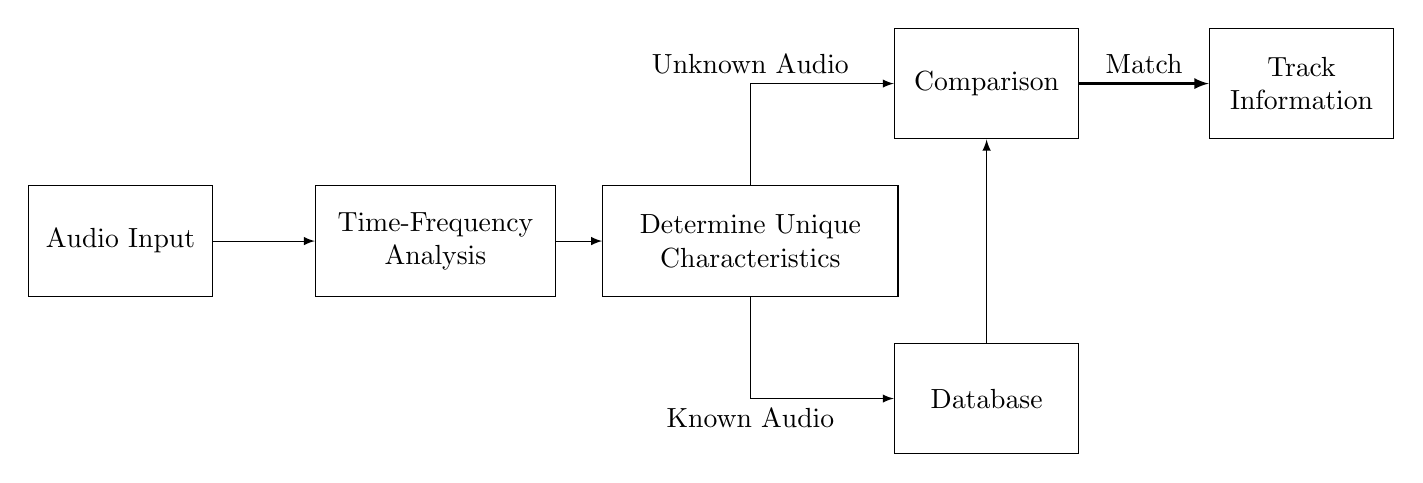
\begin{tikzpicture}[node distance =4cm, auto]
\node (AudioInput) [block]{Audio Input};
\node (TimeFreq) [block, right of=AudioInput,text width=8em]{Time-Frequency Analysis};


\node (PCA) [block, right of=TimeFreq, text width=10em]{Determine Unique Characteristics};


\coordinate [right of=PCA, node distance=3cm](T1);
%Above
\node (Comparison)[block, above of=T1, node distance=2cm]{Comparison};
\node (TrackInfo)[block, right of=Comparison]{Track Information};

%Below
\node (Database)[block, below of=T1, node distance=2cm]{Database};


\path [line](AudioInput)--(TimeFreq);
\path [line](TimeFreq)--(PCA);

\path [line](PCA)|-node[description, above]{Unknown Audio}(Comparison);
\path [line,thick](Comparison)--node[description, above]{Match}(TrackInfo);
\path [line](PCA)|-node[description, below]{Known Audio}(Database);
\path [line](Database)--(Comparison);

\end{tikzpicture}}
    \caption{A flowchart of how the system will be set up.}
    \label{fig:system_flowchart}
\end{figure}

As seen in the flowchart, the first three steps of the algorithm are the same, when using known audio or unknown audio. To analyse audio with respect to both the time and the frequency domain the theory of discrete short time Fourier transform can be used, which will transform the audio into the frequency domain which can be represented as a matrix.
To determine the unique characteristics of this matrix, principal component analysis can be used. With the use of principal component analysis, an audio fingerprint of the audio is generated. As seen in the flowchart, when having a known audio recording the fingerprints are stored in a database together with the track information. When having an unknown audio recording as an input, the data from the database is used to compare the unknown audio with known audio. If the fingerprint from the unknown audio is matched with a fingerprint in the database, the track information is presented.\\

One of the challenges of the system when analysing an unknown audio recording is that it often contains noise. Noise can be an issue since it can alter the audio, such that the fingerprint generated will differ from the fingerprint of the original signal. It could be relevant to test how much noise there could be added onto the audio before the system cannot match the audio correctly.

\section{Problem Statement}
How robust can an audio fingerprinting algorithm be constructed to recognise audio input even with noise? 

